
\documentclass[11pt, a4paper]{article}
%\usepackage{proj1}
\usepackage{natbib}
\usepackage{fancyhdr}  
\usepackage{subcaption}
\usepackage{caption}
\usepackage{graphicx}
\usepackage{numprint}
\usepackage{multirow}
\linespread{1.25} 
\setlength{\parindent}{0cm}
\graphicspath{{Images/}}
\usepackage{hyperref}
\usepackage{amsmath}
\usepackage{amsfonts}
\usepackage{amssymb}
\usepackage{amsthm}
\usepackage{mathtools}
\usepackage{commath}
\usepackage{bbm}

%\usepackage[sc,osf]{mathpazo}
\usepackage{subcaption}
\usepackage[a4paper, top=1in, left=1.0in, right=1.0in, bottom=1in, includehead, includefoot]{geometry} %Usually have top as 1in

\usepackage{listings}
\usepackage{color} %red, green, blue, yellow, cyan, magenta, black, white
\definecolor{mygreen}{RGB}{28,172,0} % color values Red, Green, Blue
\definecolor{mylilas}{RGB}{170,55,241}


\hypersetup{colorlinks,linkcolor={black},citecolor={blue},urlcolor={black}}
\usepackage{color}
\urlstyle{same}


\theoremstyle{definition}
\newtheorem{definition}{Definition}[section]

\newcommand{\adja}{q_a}
\newcommand{\adjb}{q_b}
\newcommand{\adjaB}{q_{a,\partial \Omega}}
\newcommand{\adjbB}{q_{b,\partial \Omega}}
\newcommand{\adjB}{q_{\partial \Omega}}
\newcommand{\Adja}{\mathbf{p}}
\newcommand{\Adjb}{q}
\newcommand{\adj}{q}
\newcommand{\Adjc}{{q}_{\partial \Omega}}
\newcommand{\ra}{\rho_a}
\newcommand{\rb}{\rho_b}
\newcommand{\w}{\mathbf{w}}
\newcommand{\f}{\mathbf{f}}
\newcommand{\ve}{\mathbf{v}}
\newcommand{\n}{\mathbf{n}}
\newcommand{\h}{\mathbf{h}}
\newcommand{\K}{\mathbf{K}}
\newcommand{\hr}{\widehat \rho}
\newcommand{\jf}{\mathbf j}

\DeclareMathOperator{\sgn}{sgn}
\DeclareMathOperator{\Grad}{Grad}
\DeclareMathOperator{\Div}{Div}
\DeclareMathOperator{\Lap}{Lap}
%	\begin{figure}[h]
%		\centering
%		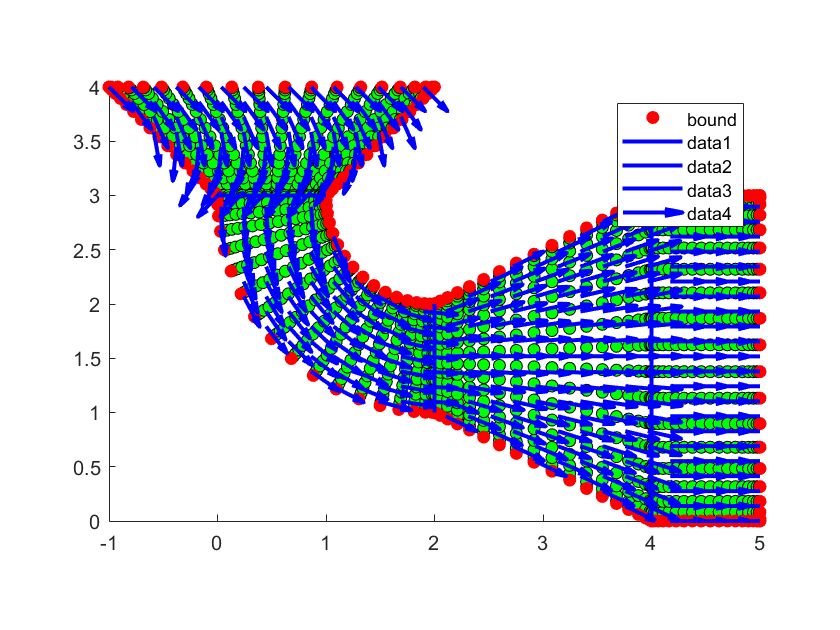
\includegraphics[scale=0.35]{F1.png}
%		\caption{Forward $\rho$ for $a = 0.01$} 
%		\label{F1}
%	\end{figure}

% \item [$\square$]

\begin{document}

	\begin{table}
\centering
\begin{tabular}{ | c | c || c | c | c | c | c ||}
\hline
\multicolumn{2}{|c||}{}& $\beta = 10^{-5}$ & $\beta = 10^{-3}$ & $\beta = 10^{-1}$ & $\beta = 10^{1}$ & $\beta = 10^{3}$  \\
\hline
\hline
\multirow{2}{*}{$\kappa= \numprint{0}$}  & $\mathcal{J}_{uc}$ & $\numprint{2.67e-2}$ & $\numprint{2.67e-2}$ & $\numprint{2.67e-2}$ & $\numprint{2.67e-2}$ & $\numprint{2.67e-2}$\\
 & $\mathcal{J}_c$ & $\numprint{8.23e-5}$ & $\numprint{3.87e-3}$ & $\numprint{2.50e-2}$ & $\numprint{2.67e-2}$ & $\numprint{2.67e-2}$\\
\hline
\multirow{2}{*}{$\kappa= \numprint{1}$}  & $\mathcal{J}_{uc}$ & $\numprint{3.29e-2}$ & $\numprint{3.29e-2}$ & $\numprint{3.29e-2}$ & $\numprint{3.29e-2}$ & $\numprint{3.29e-2}$\\
 & $\mathcal{J}_c$ & $\numprint{1.16e-4}$ & $\numprint{5.44e-3}$ & $\numprint{3.13e-2}$ & $\numprint{3.29e-2}$ & $\numprint{3.29e-2}$\\
\hline
\multirow{2}{*}{$\kappa= \numprint{-1}$}  & $\mathcal{J}_{uc}$ & $\numprint{2.09e-2}$ & $\numprint{2.09e-2}$ & $\numprint{2.09e-2}$ & $\numprint{2.09e-2}$ & $\numprint{2.09e-2}$\\
 & $\mathcal{J}_c$ & $\numprint{5.71e-5}$ & $\numprint{2.63e-3}$ & $\numprint{1.92e-2}$ & $\numprint{2.09e-2}$ & $\numprint{2.09e-2}$\\
\hline
\end{tabular}
\caption{Flow Control No-Flux Problem: Cost when $\vec{w}=\vec{0}$ and optimal control cost for a range of $\kappa$, $\beta$. Note that for $\beta = 10$, the cost functionals differ by $10^{-5}$, while for $\beta = 10^3$ they differ by $10^{-7}$ (++ two in the wrong direction ++).}
\label{TabFCN}
\end{table}
	\begin{table}
\centering
\begin{tabular}{ | c | c || c | c | c | c | c ||}
\hline
\multicolumn{2}{|c||}{}& $\beta = 10^{-5}$ & $\beta = 10^{-3}$ & $\beta = 10^{-1}$ & $\beta = 10^{1}$ & $\beta = 10^{3}$  \\
\hline
\hline
\multirow{2}{*}{$\kappa= \numprint{0}$}  & $\mathcal{J}_{uc}$ & $\numprint{0.1585}$ & $\numprint{0.1585}$ & $\numprint{0.1585}$ & $\numprint{0.1585}$ & $\numprint{0.1585}$\\
 & $\mathcal{J}_c$ & $\numprint{0.0004}$ & $\numprint{0.0077}$ & $\numprint{0.1302}$ & $\numprint{0.1582}$ & $\numprint{0.1585}$\\
\hline
\multirow{2}{*}{$\kappa= \numprint{1}$}  & $\mathcal{J}_{uc}$ & $\numprint{0.2124}$ & $\numprint{0.2124}$ & $\numprint{0.2124}$ & $\numprint{0.2124}$ & $\numprint{0.2124}$\\
 & $\mathcal{J}_c$ & $\numprint{0.0004}$ & $\numprint{0.0103}$ & $\numprint{0.1852}$ & $\numprint{0.2121}$ & $\numprint{0.2124}$\\
\hline
\multirow{2}{*}{$\kappa= \numprint{-1}$}  & $\mathcal{J}_{uc}$ & $\numprint{0.4031}$ & $\numprint{0.4031}$ & $\numprint{0.4031}$ & $\numprint{0.4031}$ & $\numprint{0.4031}$\\
 & $\mathcal{J}_c$ & $\numprint{0.0005}$ & $\numprint{0.0086}$ & $\numprint{0.1739}$ & $\numprint{0.3867}$ & $\numprint{0.4029}$\\
\hline
\end{tabular}
\caption{Flow Control Dirichlet Problem: Cost when $w=0$ and optimal control cost for a range of $\kappa$, $\beta$. For $\beta = 10$, the cost functionals differ by $10^-4$ for $\kappa = 0$ and $\kappa = 1$ and by $10^-2$ for $\kappa = -1$. For $\beta = 10^3$, the cost functionals differ by $10^{-7}$ for $\kappa = 0$, by $10^{-6}$ for $\kappa = 1$, and by $10^{-4}$ for $\kappa = -1$.}
\label{TabFCD}
\end{table}
	\begin{table}
\centering
\begin{tabular}{ | c | c || c | c | c | c | c ||}
\hline
\multicolumn{2}{|c||}{}& $\beta = 10^{-5}$ & $\beta = 10^{-3}$ & $\beta = 10^{-1}$ & $\beta = 10^{1}$ & $\beta = 10^{3}$  \\
\hline
\hline
\multirow{2}{*}{$\kappa= \numprint{0}$}  & $\mathcal{J}_{uc}$ & $\numprint{1.90e-2}$ & $\numprint{1.90e-2}$ & $\numprint{1.90e-2}$ & $\numprint{1.90e-2}$ & $\numprint{1.90e-2}$\\
 & $\mathcal{J}_c$ & $\numprint{1.29e-5}$ & $\numprint{6.65e-4}$ & $\numprint{1.37e-2}$ & $\numprint{1.89e-2}$ & $\numprint{1.90e-2}$\\
\hline
\multirow{2}{*}{$\kappa= \numprint{1}$}  & $\mathcal{J}_{uc}$ & $\numprint{1.94e-2}$ & $\numprint{1.94e-2}$ & $\numprint{1.94e-2}$ & $\numprint{1.94e-2}$ & $\numprint{1.94e-2}$\\
 & $\mathcal{J}_c$ & $\numprint{1.59e-5}$ & $\numprint{7.43e-4}$ & $\numprint{1.42e-2}$ & $\numprint{1.93e-2}$ & $\numprint{1.94e-2}$\\
\hline
\multirow{2}{*}{$\kappa= \numprint{-1}$}  & $\mathcal{J}_{uc}$ & $\numprint{2.03e-2}$ & $\numprint{2.03e-2}$ & $\numprint{2.03e-2}$ & $\numprint{2.03e-2}$ & $\numprint{2.03e-2}$\\
 & $\mathcal{J}_c$ & $\numprint{1.93e-5}$ & $\numprint{8.17e-4}$ & $\numprint{1.45e-2}$ & $\numprint{2.02e-2}$ & $\numprint{2.03e-2}$\\
\hline
\end{tabular}
\caption{Source Control No-Flux Problem: Cost when $w=0$ and optimal control cost for a range of $\kappa$, $\beta$. The value of $\mathcal J_{c}$ for $\beta = 10^{-5}$ is of order $10^{-5}$. Note that for $\beta = 10$, the cost functionals differ by $10^{-4}$, while for $\beta = 10^3$ they differ by $10^{-7}$.}
\label{TabSCN}
\end{table}
	\begin{table}
\centering
\begin{tabular}{ | c | c || c | c | c | c | c ||}
\hline
\multicolumn{2}{|c||}{}& $\beta = 10^{-5}$ & $\beta = 10^{-3}$ & $\beta = 10^{-1}$ & $\beta = 10^{1}$ & $\beta = 10^{3}$  \\
\hline
\hline
\multirow{2}{*}{$\kappa= \numprint{0}$}  & $\mathcal{J}_{uc}$ & $\numprint{1.50e-2}$ & $\numprint{1.50e-2}$ & $\numprint{1.50e-2}$ & $\numprint{1.50e-2}$ & $\numprint{1.50e-2}$\\
 & $\mathcal{J}_c$ & $\numprint{3.40e-5}$ & $\numprint{1.92e-3}$ & $\numprint{1.36e-2}$ & $\numprint{1.50e-2}$ & $\numprint{1.50e-2}$\\
\hline
\multirow{2}{*}{$\kappa= \numprint{1}$}  & $\mathcal{J}_{uc}$ & $\numprint{2.06e-2}$ & $\numprint{2.06e-2}$ & $\numprint{2.06e-2}$ & $\numprint{2.06e-2}$ & $\numprint{2.06e-2}$\\
 & $\mathcal{J}_c$ & $\numprint{4.27e-5}$ & $\numprint{2.49e-3}$ & $\numprint{1.85e-2}$ & $\numprint{2.06e-2}$ & $\numprint{2.06e-2}$\\
\hline
\multirow{2}{*}{$\kappa= \numprint{-1}$}  & $\mathcal{J}_{uc}$ & $\numprint{1.27e-2}$ & $\numprint{1.27e-2}$ & $\numprint{1.27e-2}$ & $\numprint{1.27e-2}$ & $\numprint{1.27e-2}$\\
 & $\mathcal{J}_c$ & $\numprint{2.88e-5}$ & $\numprint{1.61e-3}$ & $\numprint{1.18e-2}$ & $\numprint{1.27e-2}$ & $\numprint{1.27e-2}$\\
\hline
\end{tabular}
\caption{Source Control Dirichlet Problem: Cost $\mathcal{J}_{uc}$ of applying no control (i.e., $\vec{w} = \vec{0}$)and optimal control cost $\mathcal{J}_{c}$ for a range of values of the interaction strength $\kappa$ and regularization parameter $\beta$. The value of $\mathcal J_{c}$ for $\beta = 10^{-5}$ is of order $10^{-5}$. Note that for $\beta = 10$, the cost functionals differ by $10{-5}$, while for $\beta = 10^3$ they differ by $10^{-7}$ for $\kappa = 0$ and $\kappa = 1$ and by $10^{-8}$ for $\kappa = -1$.}
\label{TabSCD}
\end{table}
	
\end{document}